%---------------------------------------------------------------
\subsection{Architecture}
\begin{frame}[t]{Architecture: Overview}
	\begin{enumerate}
		\item Records the user requests
		\item Tracks the dependencies between requests using the database
		\item Loads a snapshot
		\item Replays the legitimate user requests
	\end{enumerate}
\end{frame}

\begin{frame}[t]{Architecture: Recording}
	\begin{center}
		\vskip-20pt 
		\begin{figure} 
		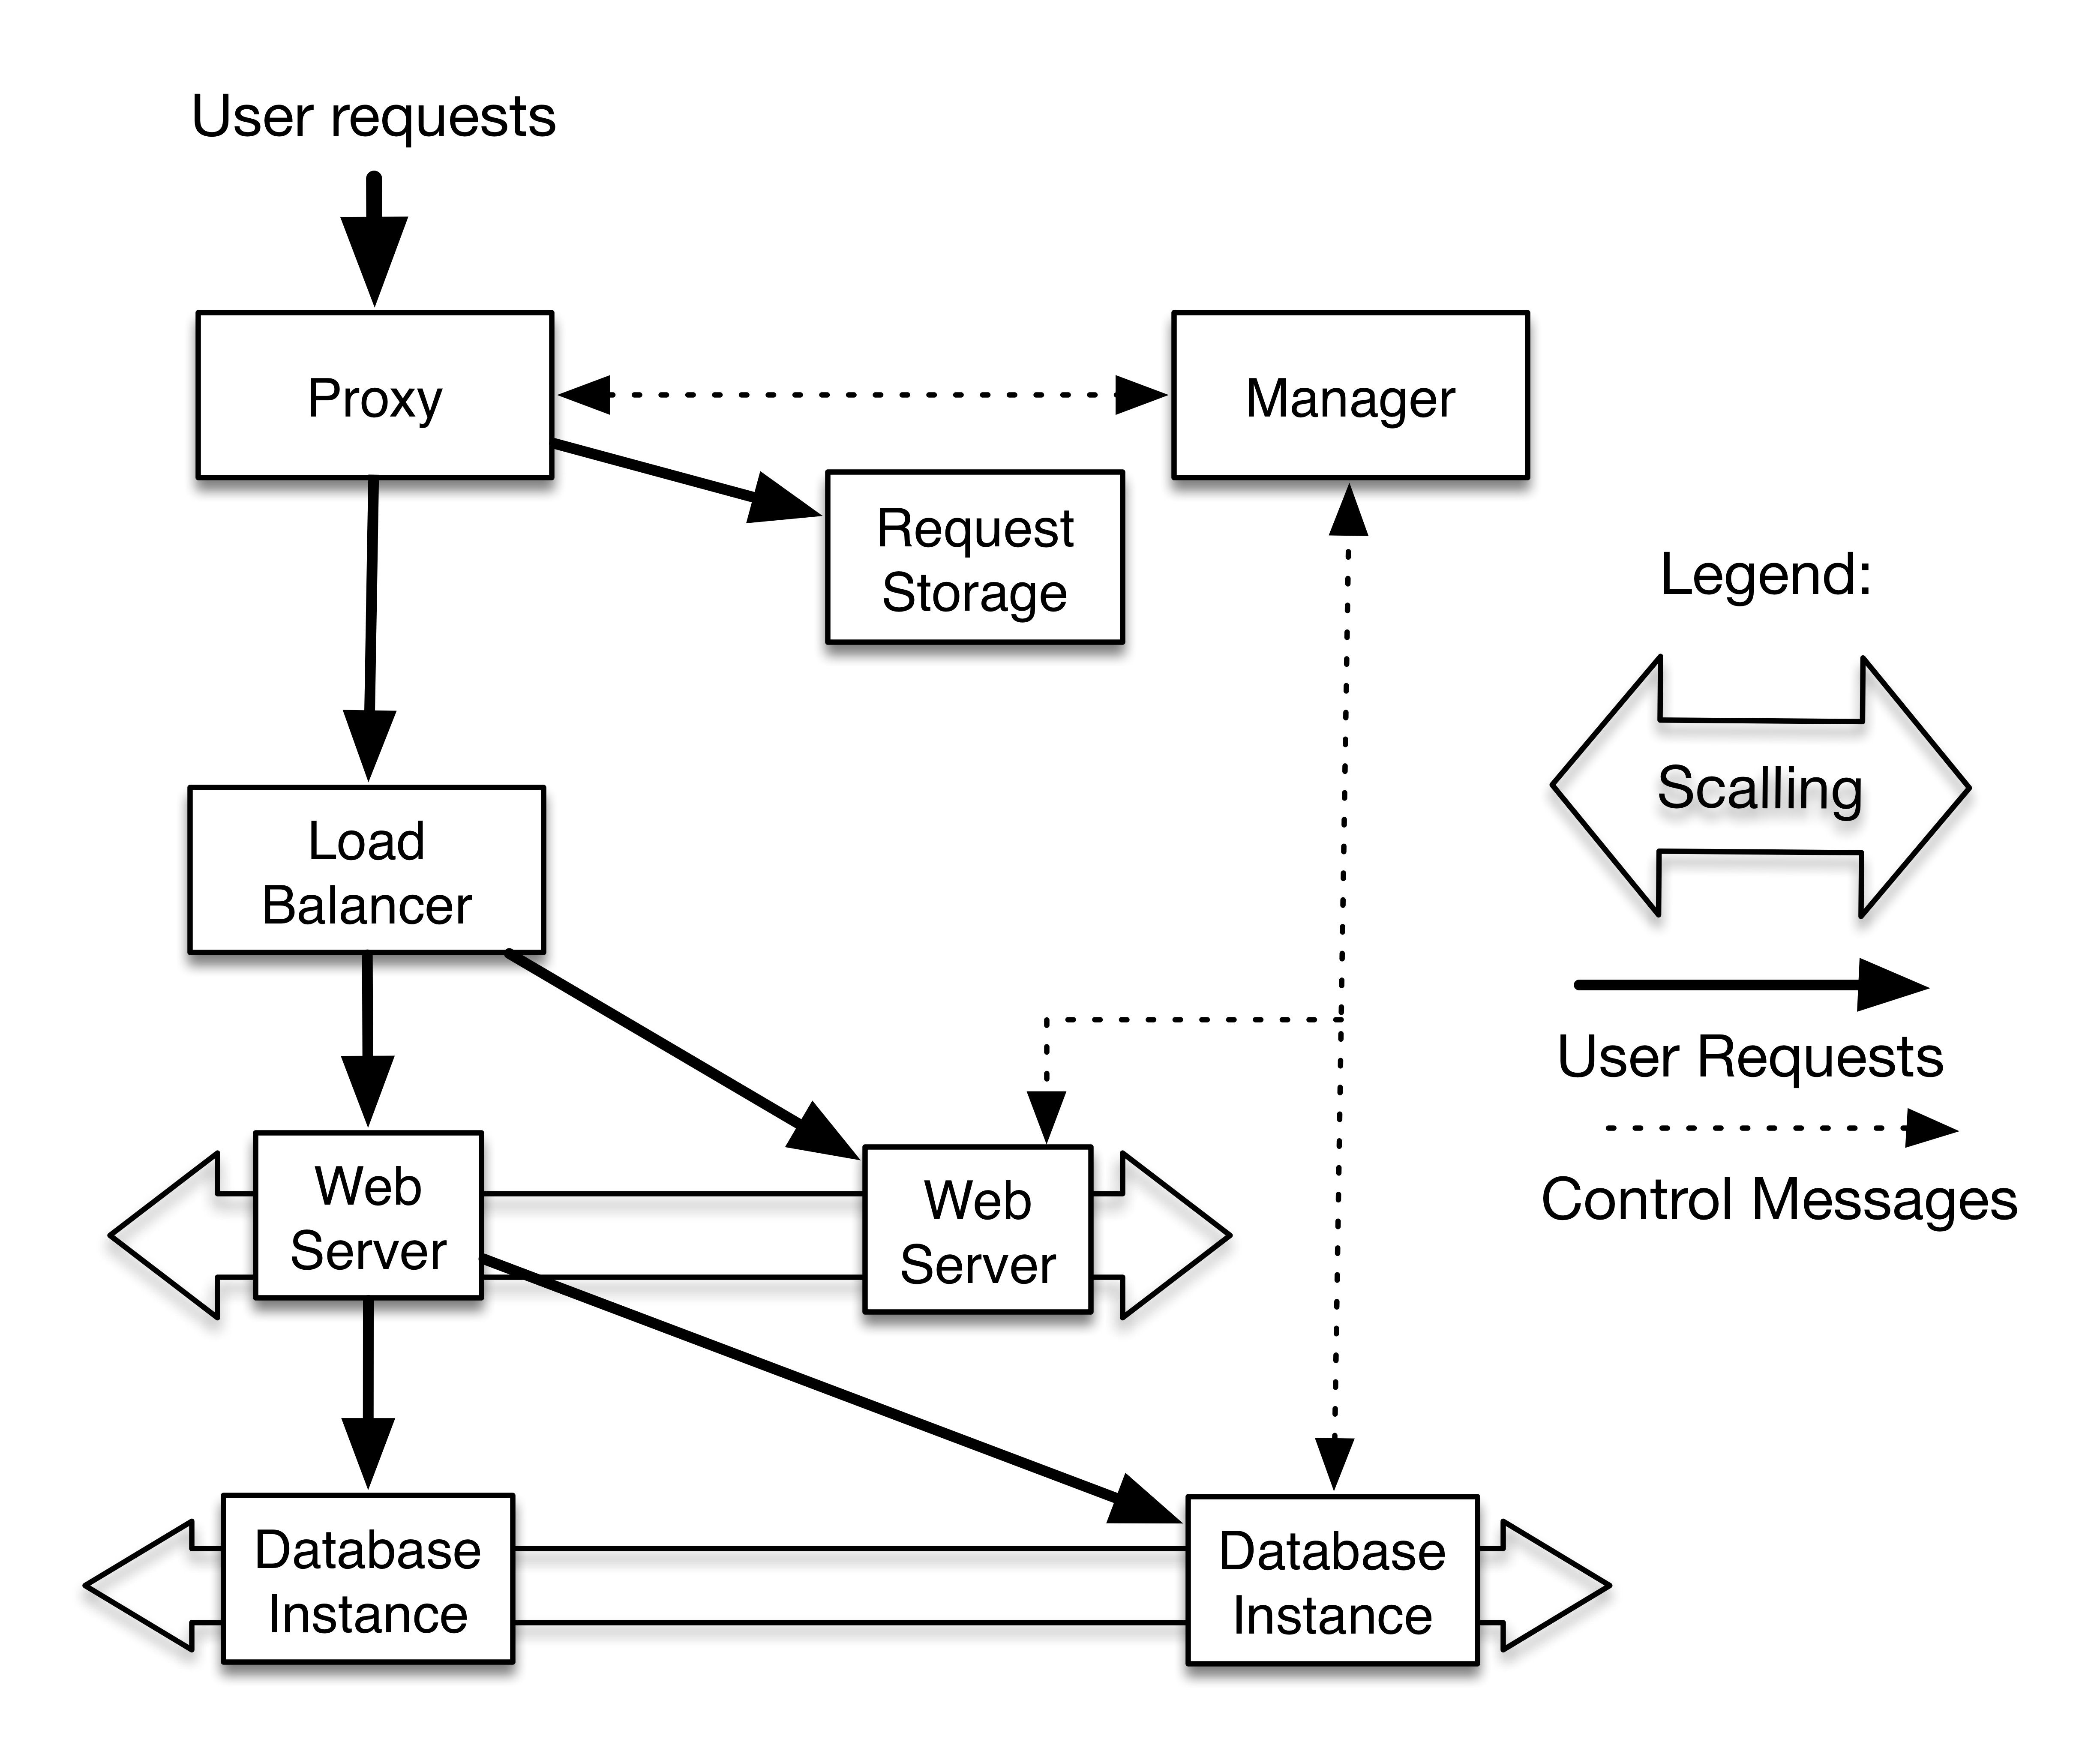
\includegraphics[width=0.8\textwidth]{img/architectureRecord}
		\end{figure}
	\end{center}
	
\note{
A arquitectura tira proveito do modelo PaaS. Usamos um proxy HTTP que antecede o load-balancer para registar os pedidos do utilizador de modo independente da aplicação. Os pedidos são marcados com um timestamp e depois guardados numa base de dados escalável e a sua identificação é enviada ao manager.
Os pedidos são depois distribuidos pela camada aplicacional que faz invocações à base de dados.
Cada nó do webserver regista os objectos acedidos por cada pedido. Depois, cada objecto da base de dados regista a ordem pela qual os pedidos lhe acedem. Estes metadados sao enviados ao manager para gerar o grafo de dependencias.
} 
\end{frame}


%------------------
\begin{frame}[t]{Architecture: Recovery}  
	\vskip-0.7cm
	\begin{enumerate}
		\setlength{\wideitemsep}{0.2cm}
		\item Load a previous snapshot in background
		\item Get the requests order using the graph
		\item Send the requests in parallel using the replay nodes
	\end{enumerate}
	\vskip-0.3cm
	\begin{center}
		\begin{figure} 
		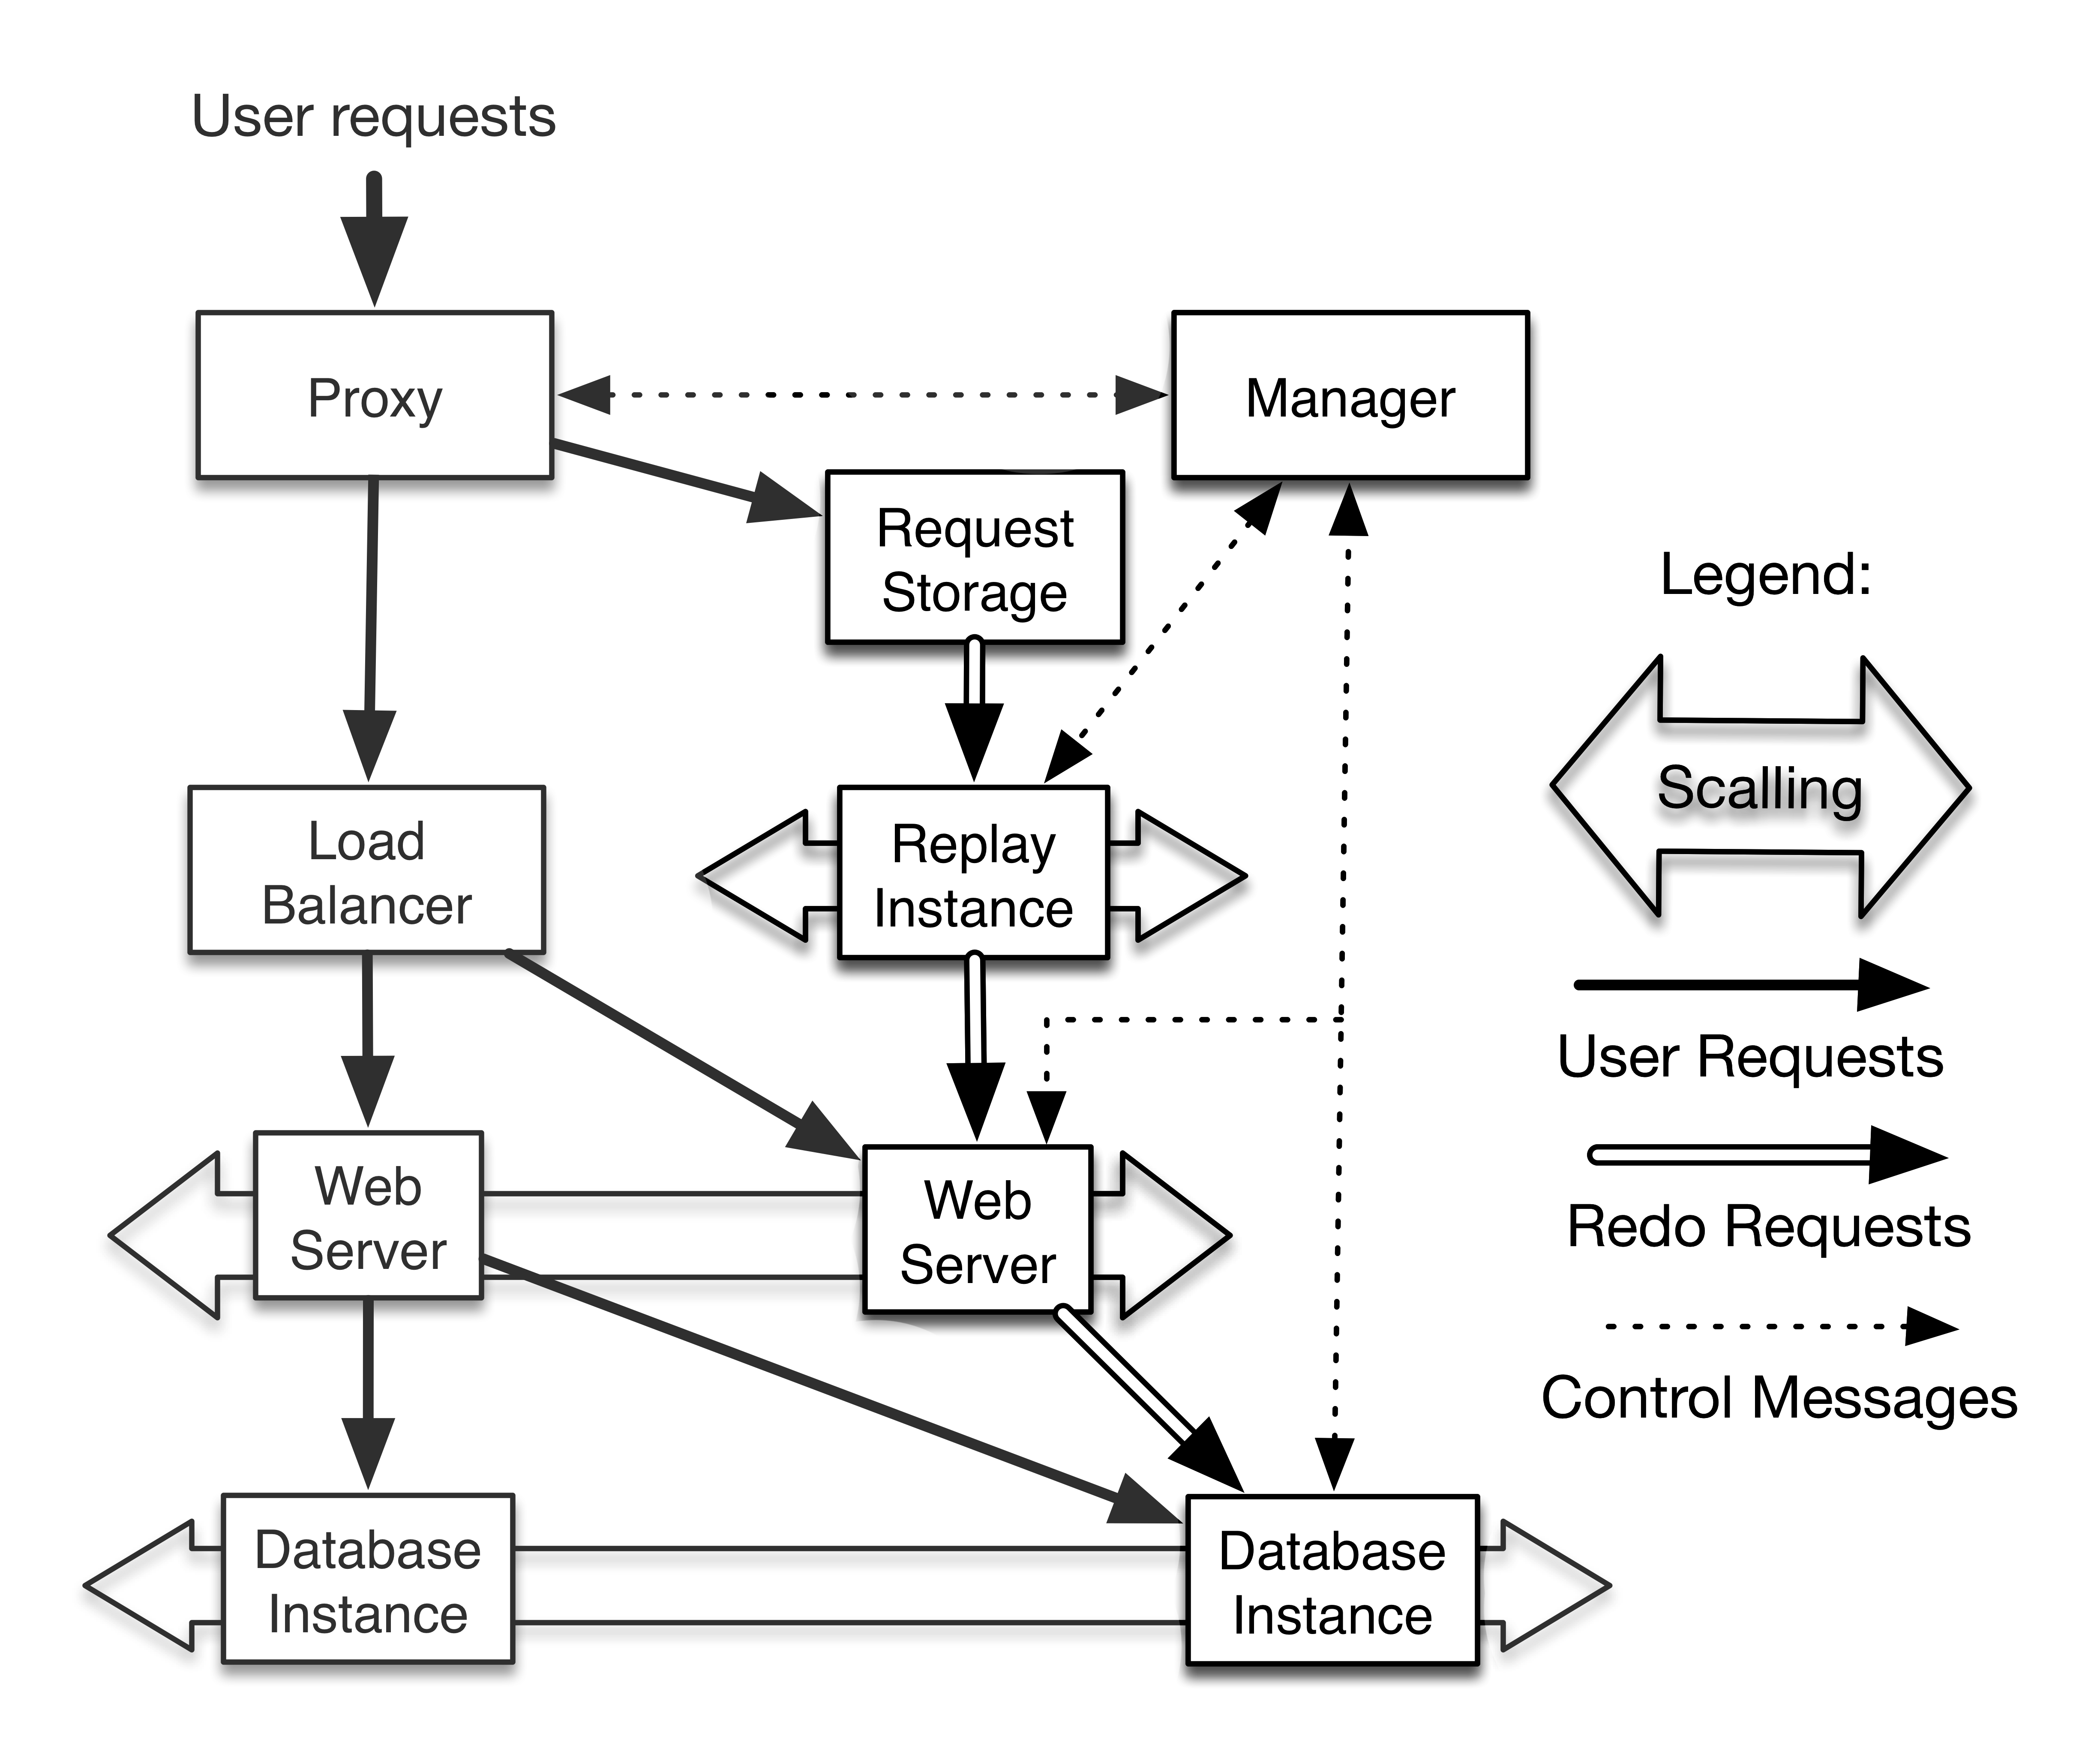
\includegraphics[width=0.65\textwidth]{img/architectureReplay}
		\end{figure}
	\end{center}
	
\end{frame}


%------------------
\begin{frame}[t]{Architecture: PaaS}
	\begin{itemize}
		\item PaaS controller lunches new database and application instances
		\item Clean images: replace corrupted instances
		\item Pay-per-use model
		\item Virtually unlimited computing and storage resources
	\end{itemize}
\end{frame}

%------------------


\begin{frame}[t]{Architecture: Branching}
\begin{columns}
\column{.7\textwidth}
	\begin{itemize}
		\item Support multiple recovery branches
		\item The branch is defined by the request header
	\end{itemize}

	\column{.3\textwidth}
		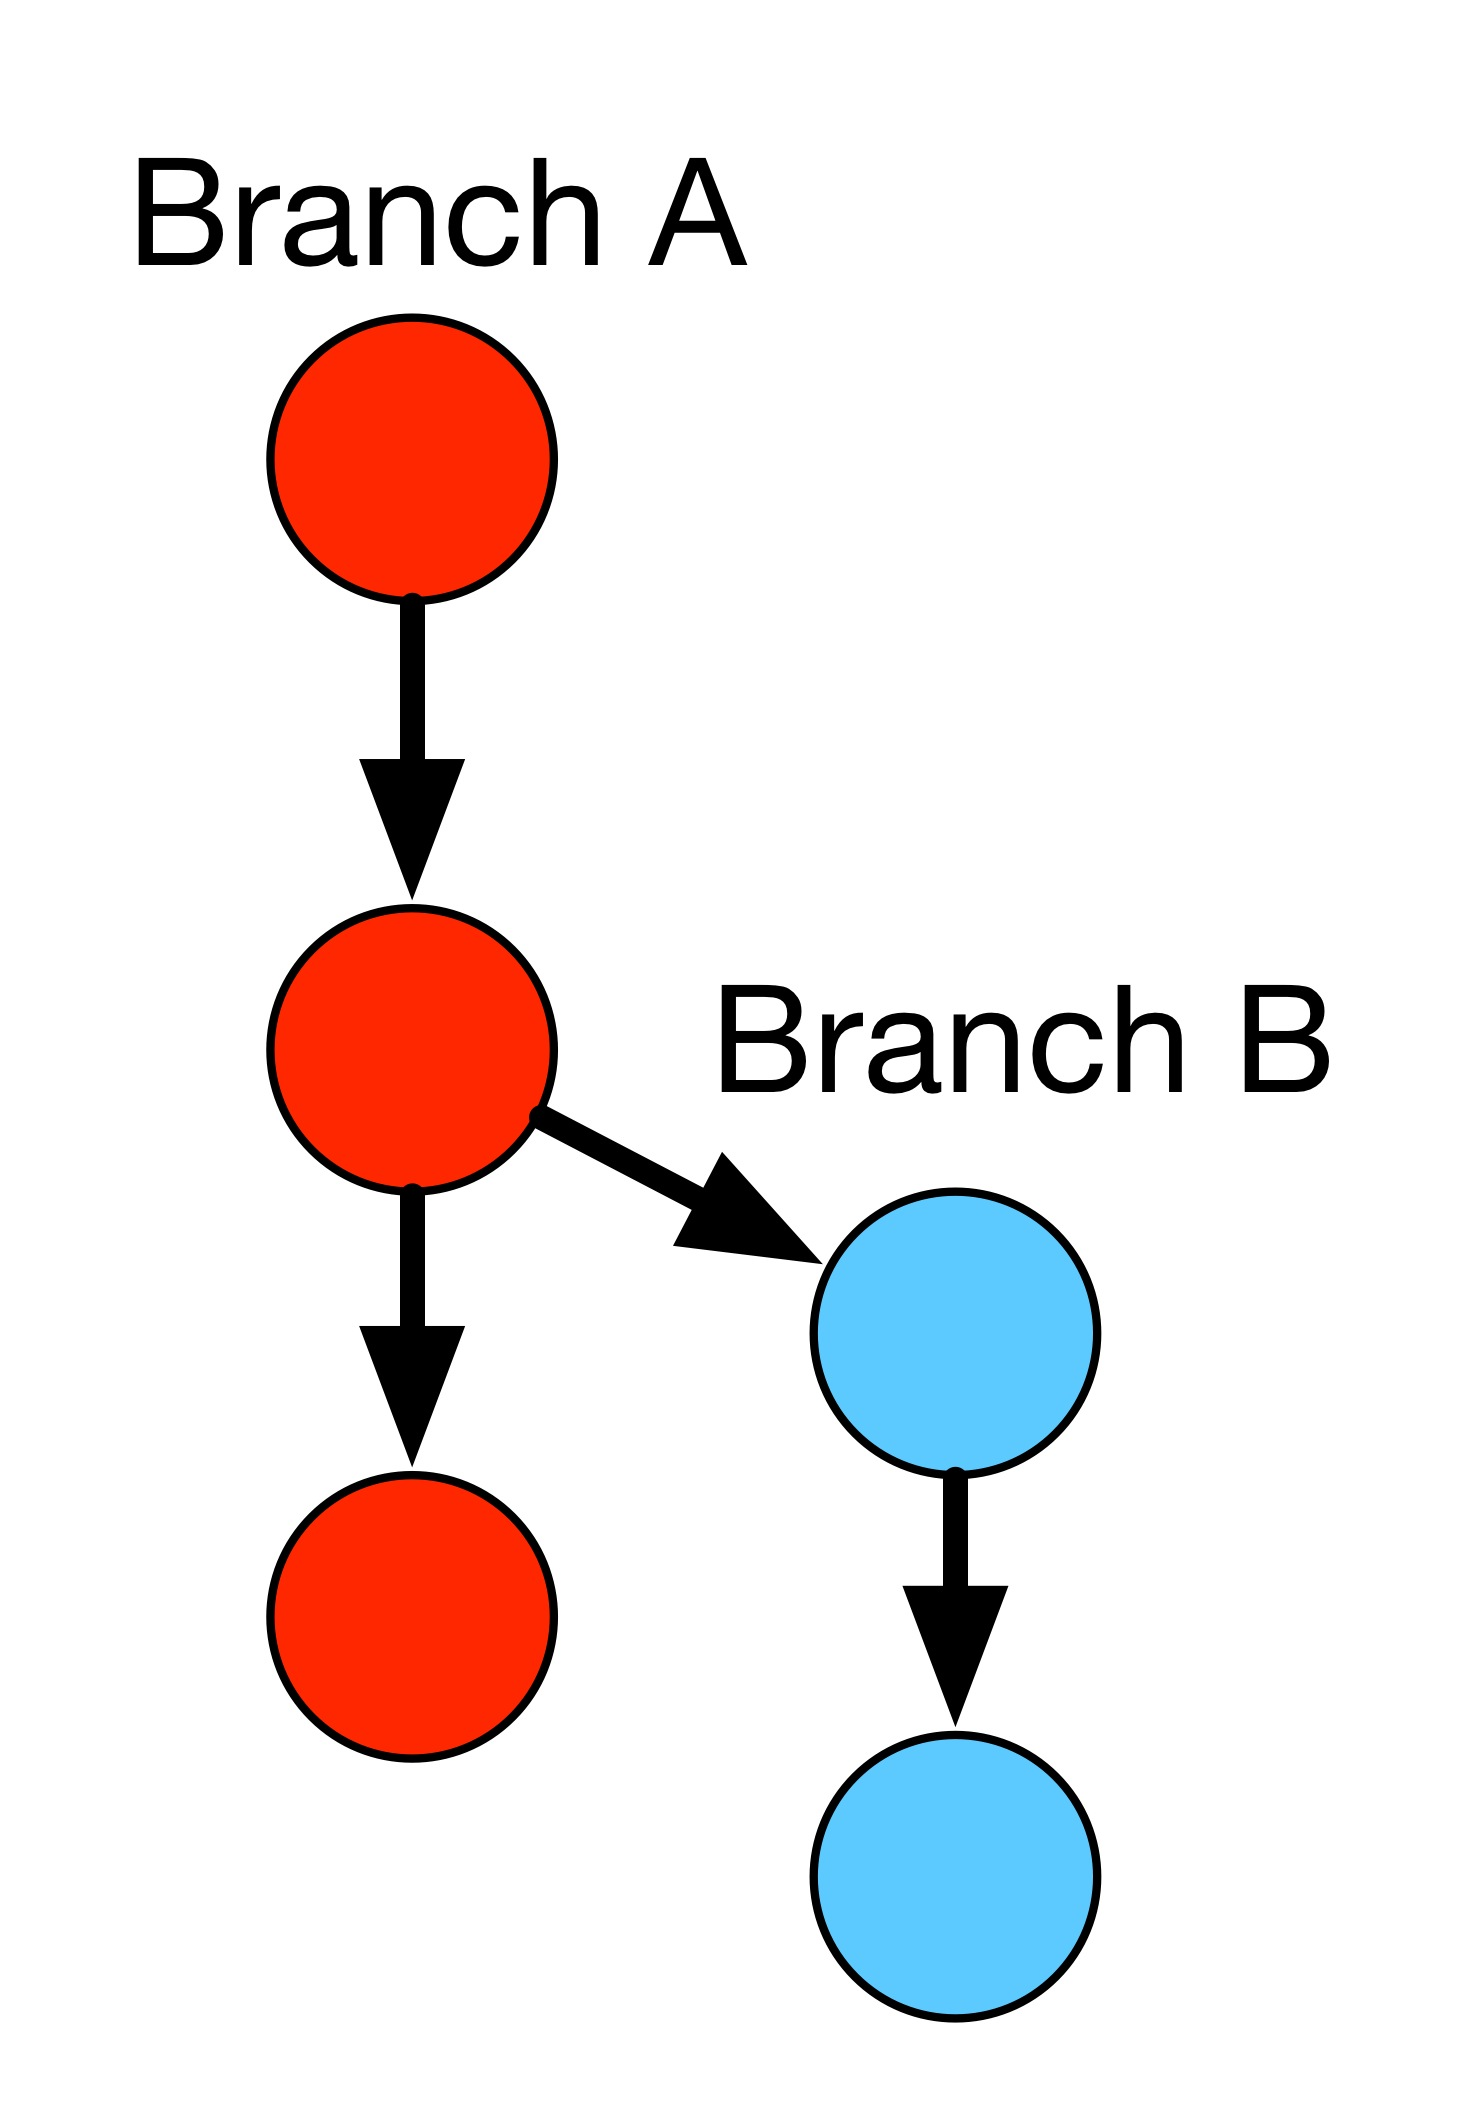
\includegraphics[width=\textwidth]{img/branch}
\end{columns}
	
\note{
Para suportar que o administrador possa visualizar os resultados da recuperação antes dos expor, o manager define em que branch é que os pedidos vão ser escritos. Para os pedidos dos utilizadores, o proxy coloca no header o branch. Para os pedidos de replay, o replay node coloca o header.
} 
\end{frame}